\section{Analyse en composante principale}

	\subsection{Le principe}

  Les d�tails math�matiques ne seront pas pr�sent�s. Il s'agit juste de montrer
  comment on peut synth�tiser un probl�me avec des variables artificielles
  dont le nombre est inf�rieur ou tr�s inf�rieure au nombre de variables
  initiales qui d�crivent les individus.
  

	\subsection{Temp�rature}

\begin{knitrout}\footnotesize
\definecolor{shadecolor}{rgb}{0.969, 0.969, 0.969}\color{fgcolor}\begin{kframe}
\begin{alltt}
\hlstd{temp} \hlkwb{<-} \hlkwd{read.csv2}\hlstd{(}\hlstr{"data/temp.csv"}\hlstd{)}
\hlkwd{colnames}\hlstd{(temp)}
\end{alltt}
\begin{verbatim}
##  [1] "Ville"     "Janvier"   "Fevrier"  
##  [4] "Mars"      "Avril"     "Mai"      
##  [7] "Juin"      "Juillet"   "Aout"     
## [10] "Septembre" "Octobre"   "Novembre" 
## [13] "Decembre"  "lati"      "long"
\end{verbatim}
\end{kframe}
\end{knitrout}



\begin{knitrout}\footnotesize
\definecolor{shadecolor}{rgb}{0.969, 0.969, 0.969}\color{fgcolor}\begin{kframe}
\begin{alltt}
\hlkwd{head}\hlstd{(temp)}
\end{alltt}
\begin{verbatim}
##              Ville Janvier Fevrier Mars Avril
## 1         Bordeaux     5.6     6.6 10.3  12.8
## 2            Brest     6.1     5.8  7.8   9.2
## 3 Clermont-Ferrand     2.6     3.7  7.5  10.3
## 4         Grenoble     1.5     3.2  7.7  10.6
## 5            Lille     2.4     2.9  6.0   8.9
## 6             Lyon     2.1     3.3  7.7  10.9
##    Mai Juin Juillet Aout Septembre Octobre
## 1 15.8 19.3    20.9 21.0      18.6    13.8
## 2 11.6 14.4    15.6 16.0      14.7    12.0
## 3 13.8 17.3    19.4 19.1      16.2    11.2
## 4 14.5 17.8    20.1 19.5      16.7    11.4
## 5 12.4 15.3    17.1 17.1      14.7    10.4
## 6 14.9 18.5    20.7 20.1      16.9    11.4
##   Novembre Decembre  lati  long
## 1      9.1      6.2 44.50 -0.34
## 2      9.0      7.0 48.24 -4.29
## 3      6.6      3.6 45.47  3.05
## 4      6.5      2.3 45.10  5.43
## 5      6.1      3.5 50.38  3.04
## 6      6.7      3.1 45.45  4.51
\end{verbatim}
\end{kframe}
\end{knitrout}


	\subsection{Les donn�es}
	
	Ce sont donc les donn�es qui correspondent aux temp�ratures moyennes
	tout au long de l'ann�e pour des villes de France.


  \subsection{Peut-on r�sumer les informations ?}

Le principe de l'ACP est de chercher et de simplifier les corr�lations qui existe
entre les variables pour cr�er des variables synth�tiques qui avec peu 
de nouvelles variables r�sumeront le maximum d'informations possibles.

Pour r�aliser l'analyse on utilise le paquet FactoMineR.


	\subsection{Pr�paration des donn�es}

\begin{knitrout}\footnotesize
\definecolor{shadecolor}{rgb}{0.969, 0.969, 0.969}\color{fgcolor}\begin{kframe}
\begin{alltt}
\hlkwd{rownames}\hlstd{(temp)} \hlkwb{<-} \hlstd{temp}\hlopt{$}\hlstd{Ville}
\hlstd{temp} \hlkwb{<-} \hlstd{temp[,}\hlopt{-}\hlnum{1}\hlstd{]}
\end{alltt}
\end{kframe}
\end{knitrout}


  \subsection{Graphiques des variables}

\begin{knitrout}\footnotesize
\definecolor{shadecolor}{rgb}{0.969, 0.969, 0.969}\color{fgcolor}\begin{kframe}
\begin{alltt}
\hlstd{pca} \hlkwb{<-} \hlkwd{PCA}\hlstd{(temp,}\hlkwc{quanti.sup} \hlstd{=} \hlkwd{c}\hlstd{(}\hlnum{13}\hlstd{,}\hlnum{14}\hlstd{))}
\end{alltt}
\end{kframe}

{\centering 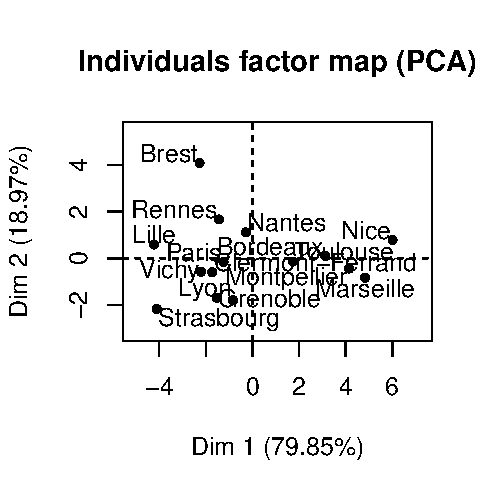
\includegraphics[width=\textwidth]{graphiques/beamer-unnamed-chunk-5-1} 
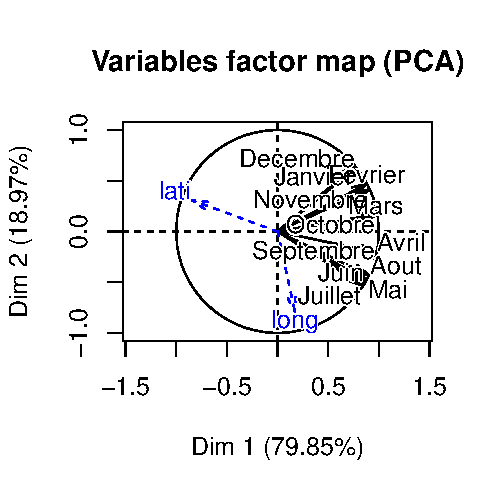
\includegraphics[width=\textwidth]{graphiques/beamer-unnamed-chunk-5-2} 

}



\end{knitrout}

colnames(temp)  
  

  \subsection{Graphique des  individus sur les deux premiers axes}

\begin{knitrout}\footnotesize
\definecolor{shadecolor}{rgb}{0.969, 0.969, 0.969}\color{fgcolor}\begin{kframe}
\begin{alltt}
\hlkwd{plot}\hlstd{(pca,}\hlkwc{choix} \hlstd{=} \hlstr{"ind"}\hlstd{)}
\end{alltt}
\end{kframe}

{\centering 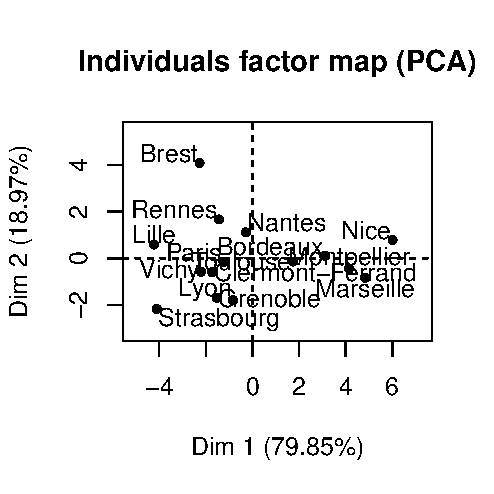
\includegraphics[width=\textwidth]{graphiques/beamer-unnamed-chunk-6-1} 

}



\end{knitrout}




\begin{knitrout}\footnotesize
\definecolor{shadecolor}{rgb}{0.969, 0.969, 0.969}\color{fgcolor}\begin{kframe}
\begin{alltt}
\hlkwd{cor}\hlstd{(pca}\hlopt{$}\hlstd{ind}\hlopt{$}\hlstd{coord[,}\hlnum{1}\hlopt{:}\hlnum{2}\hlstd{],temp[,}\hlkwd{c}\hlstd{(}\hlstr{"lati"}\hlstd{,}\hlstr{"long"}\hlstd{)])}
\end{alltt}
\begin{verbatim}
##             lati       long
## Dim.1 -0.8389348  0.1714839
## Dim.2  0.3064996 -0.7922192
\end{verbatim}
\end{kframe}
\end{knitrout}


  A partir des donn�es et des r�sultats de l'ACP, nous avons pu retrouver
  la lattitude et la longitude approximative.
  



